\documentclass[xcolor=dvipsnames,notes]{beamer}
\usecolortheme[named=Brown]{structure}
\usetheme{default}
\setbeamertemplate{navigation symbols}{} 
\usepackage{tikz}
\usetikzlibrary{arrows,decorations.pathmorphing,backgrounds,positioning,fit}
\usetikzlibrary{datavisualization.formats.functions}
\usetikzlibrary{shapes}
\usetikzlibrary{calc,patterns,angles,quotes}
%     
%Here are some macro's saving time and labour:     
%     
\newcommand{\const}{\mbox{const}}      
\newcommand{\est}{\mbox{{\tiny est}}}      
\newcommand{\im}{\mbox{$\Im \mbox{m}$}}      
\newcommand{\obs}{\mbox{{\tiny obs}}}      
\newcommand{\otherwise}{\mbox{otherwise}}      
\newcommand{\real}{\mbox{$\Re \mbox{e}$}}      
\newcommand{\sign}{\mbox{sign}}      
\newcommand{\sinc}{\mbox{sinc}}      
%
\newcommand{\p}{\mbox{$\partial$}}      
\renewcommand{\d}{\mbox{$\partial$}}      
\newcommand{\w}{\mbox{$\omega$}}      
%
\newcommand{\AAA}{\mbox{\boldmath $A$}}   
\newcommand{\BB}{\mbox{\boldmath $B$}}     
\newcommand{\CC}{\mbox{\boldmath $C$}}     
\newcommand{\DD}{\mbox{\boldmath $D$}}     
\newcommand{\EE}{\mbox{\boldmath $E$}}     
\newcommand{\FF}{\mbox{\boldmath $F$}}   
\newcommand{\GG}{\mbox{\boldmath $G$}}   
\newcommand{\HH}{\mbox{\boldmath $H$}}   
\newcommand{\II}{\mbox{\boldmath $I$}}   
\newcommand{\JJ}{\mbox{\boldmath $J$}}   
\newcommand{\KK}{\mbox{\boldmath $K$}}   
\newcommand{\LL}{\mbox{\boldmath $L$}}   
\newcommand{\MM}{\mbox{\boldmath $M$}}   
\newcommand{\NN}{\mbox{\boldmath $N$}}   
\newcommand{\OO}{\mbox{\boldmath $O$}}   
\newcommand{\PP}{\mbox{\boldmath $P$}}   
\newcommand{\QQ}{\mbox{\boldmath $Q$}}   
\newcommand{\RR}{\mbox{\boldmath $R$}}   
\newcommand{\SSS}{\mbox{\boldmath $S$}}   
\newcommand{\TT}{\mbox{\boldmath $T$}}   
\newcommand{\UU}{\mbox{\boldmath $U$}}   
\newcommand{\VV}{\mbox{\boldmath $V$}}   
\newcommand{\WW}{\mbox{\boldmath $W$}}   
\newcommand{\XX}{\mbox{\boldmath $X$}}   
\newcommand{\YY}{\mbox{\boldmath $Y$}}   
\newcommand{\ZZ}{\mbox{\boldmath $Z$}}   
%
%\newcommand{\aaa}{\mbox{\boldmath $a$}}     
\newcommand{\bb}{\mbox{\boldmath $b$}}     
\newcommand{\cc}{\mbox{\boldmath $c$}}     
\newcommand{\dd}{\mbox{\boldmath $d$}}     
\newcommand{\ee}{\mbox{\boldmath $e$}}   
\newcommand{\ff}{\mbox{\boldmath $f$}}   
%\newcommand{\ggg}{\mbox{\boldmath $g$}}   
\newcommand{\hh}{\mbox{\boldmath $h$}}   
\newcommand{\ii}{\mbox{\boldmath $i$}}   
\newcommand{\jj}{\mbox{\boldmath $j$}}   
\newcommand{\kk}{\mbox{\boldmath $k$}}   
%\newcommand{\lll}{\mbox{\boldmath $l$}}   
\newcommand{\mm}{\mbox{\boldmath $m$}}   
\newcommand{\nn}{\mbox{\boldmath $n$}}   
\newcommand{\pp}{\mbox{\boldmath $p$}}   
\newcommand{\qq}{\mbox{\boldmath $q$}}   
\newcommand{\rr}{\mbox{\boldmath $r$}}   
%\newcommand{\sss}{\mbox{\boldmath $s$}}   
%\newcommand{\ttt}{\mbox{\boldmath $t$}}   
\newcommand{\uu}{\mbox{\boldmath $u$}}   
\newcommand{\vv}{\mbox{\boldmath $v$}}   
\newcommand{\ww}{\mbox{\boldmath $w$}}   
\newcommand{\xx}{\mbox{\boldmath $x$}}   
\newcommand{\yy}{\mbox{\boldmath $y$}}   
\newcommand{\zz}{\mbox{\boldmath $z$}}   
%
\newcommand{\balpha}{\mbox{\boldmath $\alpha$}}     
\newcommand{\bpsi}{\mbox{\boldmath $\psi$}}     
\newcommand{\bphi}{\mbox{\boldmath $\phi$}}     
\newcommand{\bbeta}{\mbox{\boldmath $\beta$}}     
\newcommand{\btheta}{\mbox{\boldmath $\theta$}}     
\newcommand{\bdelta}{\mbox{\boldmath $\delta$}}     
\newcommand{\bgamma}{\mbox{\boldmath $d$}}     
\newcommand{\bGamma}{\mbox{\boldmath $\Gamma$}}     
\newcommand{\bLambda}{\mbox{\boldmath $\Lambda$}}     
\newcommand{\bmu}{\mbox{\boldmath $\mu$}}     
\newcommand{\bnabla}{\mbox{\boldmath $\nabla$}}     
\newcommand{\brho}{\mbox{\boldmath $\rho$}}     
\newcommand{\bSigma}{\mbox{\boldmath $\Sigma$}}     
\newcommand{\bsigma}{\mbox{\boldmath $\sigma$}}     
\newcommand{\bxi}{\mbox{\boldmath $\xi$}}     
\newcommand{\bepsilon}{\mbox{\boldmath $\epsilon$}}     
\newcommand{\blambda}{\mbox{\boldmath $\lambda$}}     
\newcommand{\BLambda}{\mbox{\boldmath $\Lambda$}}     
%-------------------------------------%
%  \Appendix - a new appendix command %
%-------------------------------------%
%The appendix command is used as in
% \Appendix{A}{The wave equation as a matrix equation}
\newcommand {\Appendix}[1]{
              \section*{APPENDIX #1}
              \setcounter{equation}{0}
              \renewcommand{\theequation} 
              {A-\arabic{equation}}}
\newcommand {\Appendices}[2]{
              \section*{APPENDIX #1: #2 }
              \setcounter{equation}{0}
              \renewcommand{\theequation} 
              {#1-\arabic{equation}}}
%------------------------------------%
%    \aref - a new cite command.     % 
%------------------------------------%
\newcommand{\aref}[2]{\nocite{#1}#2} 
%----------------------------------------
%\eqref -an equation reference command
%----------------------------------------
%\newcommand{\eqref}[1]{(\ref{#1})}
%\newcommand{\eqref}[1]{\ref{#1}}

\usepackage{epsfig}
\usepackage{natbib}
\usepackage{graphicx}
\usepackage{multimedia}
\usepackage{verbatim}
\include{acmmacro}
\begin{document}
%\setbeamercolor{titlelike}{fg=gray,bg=white}
%\setbeamercolor{itemize item}{fg=gray,bg=white}
%\setbeamercolor{enumerate item}{fg=gray,bg=white}
%\setbeamercolor{block title}{fg=black,bg=white}
%==============================================
\title{TPG4190 Seismic data acquisition and processing \\
               Lecture 18: Multiples - Surface Related Multiple Removal (SRME)}
\author{B. Arntsen}
\institute[NTNU]{
  NTNU\\
  Department of Geoscience and petroleum \\
  \texttt{borge.arntsen@ntnu.no}
}
\date{Trondheim fall 2020}
\begin{frame}
 \titlepage
\end{frame}
%
%==============================================
\begin{frame}{Surface Related Multiple Removal (SRME)}
%==============================================
\begin{itemize}
   \item Multiple reflections generated by the sea surface are usually strong
   \item Mathematical removal of the sea surface removes surface multiples
   \item SRME does not rely on moveout discrimination
\end{itemize}
\end{frame}
%
%===================================================================
\begin{frame}{Model for multiple reflections}
%===================================================================
\begin{figure}
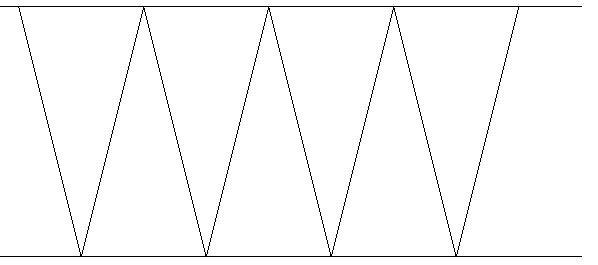
\includegraphics[width=0.6\textwidth]{Fig/mult.pdf}
\caption{Raypaths for multiple reflections}
\end{figure}
\end{frame}
%
%
\begin{frame}{Model for multiple reflections}
\begin{itemize} 
  \item Vertically traveling waves
  \item $\tau$: Traveltime
  \item $r$: Reflection coefficient at the bottom
  \item Reflection coefficient at the top is equal to -1
\end{itemize}
%
\begin{eqnarray}
 p(t) = r s(t-\tau) - r^2 s(t-2\tau) +  r^3 s(t-3\tau) + \ldots
                                \label{eq:mult}
\end{eqnarray}
\end{frame}
%
\begin{frame}{Model for multiple reflections}
Taking the Fourier transform of equation \eqref{eq:mult}, one gets
%
\begin{eqnarray}
  P(\omega) = rS(\omega)\exp(-i\omega \tau) 
   -  r^2 S(f)\exp(-2i\omega\tau) +  r^3\exp(-3i\omega \tau) 
   + \ldots \nonumber\\
                                \label{eq:fmult}
\end{eqnarray}
%
If we set $R=r\exp(-i\omega\tau)$, then equation \eqref{eq:fmult} is: 
%
\begin{eqnarray}
  P(\omega) = S(\omega)R\left[1 -  R +  R^2  + \ldots\right].
                                \label{eq:fmult2}
\end{eqnarray}
\end{frame}
%
%
\begin{frame}{Model for multiple reflections}
The right hand side of equation \eqref{eq:mult} is an infinite geometrical series,
%
\begin{eqnarray}
\frac{1}{1+x} = 1-x+x^2-x^3+\ldots
                            \label{eq:fmult2b}
\end{eqnarray}
implying 
%
\begin{eqnarray}
  P(\omega) = \frac{S(\omega)R}{1+R}.
                                \label{eq:fmult3}
\end{eqnarray}
%
\end{frame}
%
%
\begin{frame}{Removal of multiples}
%
Equation \eqref{eq:fmult3} solved with respect to $R$ 
%
\begin{eqnarray}
  R = \frac{P(\omega)}{S(\omega)[1-S^{-1}(f)P(\omega)]},
                                \label{eq:ch6-101}
\end{eqnarray}
%
or
%
\begin{eqnarray}
  S(\omega)R = \frac{P(\omega)}{[1-S^{-1}(f)P(\omega)]}.
                                \label{eq:ch6-102}
\end{eqnarray}
%
Use of (Rottmann (1960)) 
%
\begin{eqnarray}
  \frac{1}{1-x} = 1+x+x^2+x^3+\ldots,
\end{eqnarray}
gives
\end{frame}
%
%
\begin{frame}{Removal of multiples}
%
\begin{eqnarray}
  P_0(f) = P(\omega)\left[1+S^{-1}P(\omega) + S^-2P^2(\omega)+\ldots\right],
                                \label{eq:ch6-103}
\end{eqnarray}
%
where $P_0(\omega)= S(\omega)R(\omega)$ is the primary response,
\end{frame}
%
%
\begin{frame}{Removal of multiples}
\begin{itemize}
  \item Remove multiple reflections by summing powers of the recorded data itself

  \item \eqref{eq:ch6-103} does {\em not} require any knowledge of the water depth nor the
        reflection coefficient!
\end{itemize}
\end{frame}
%
%
\begin{frame}{Removal of multiples}
To see how the summation works, truncate the series 
%
\begin{eqnarray}
  P_0(\omega) \approx P(\omega)+S^{-1}P^2(\omega),
                                \label{eq:ch6-106}
\end{eqnarray}
%
and insert equation \eqref{eq:fmult3} into equation \eqref{eq:ch6-106}
%
\begin{eqnarray}
  P_0(\omega) \approx \frac{S(\omega)R(\omega)}{1+R(\omega)} + 
  S^{-1}(\omega) \frac{S^2(\omega)R^2(\omega)}{[1+R(\omega)]^2}.
                                \label{eq:ch6-107}
\end{eqnarray}
%
Using the following relations
%
\begin{eqnarray}
 \frac{1}{1+x} = 1-x+\ldots,\nonumber\\
 \frac{1}{{(1+x)}^2} = 1-2x+\ldots,\nonumber\\
\end{eqnarray}
\end{frame}
%
%
\begin{frame}{Removal of multiples}
we have
%
\begin{eqnarray}
\frac{S(\omega)R(\omega)}{1+R(\omega)} \approx S(\omega)R(\omega)\left[1-R(\omega)\right],
\end{eqnarray}
and
%
\begin{eqnarray}
S^{-1}(\omega) \frac{S^2(f)R^2(\omega)}{[1+R(\omega)]^2} 
         \approx S^{-1}(\omega) S^2(\omega)R^2(\omega){[1-2R(\omega)]},
\end{eqnarray}
%
equation \eqref{eq:ch6-107} becomes
%
\begin{eqnarray}
  P_0(\omega) \approx S(\omega)R(\omega)\left[1-R(\omega)\right] 
               + S^{-1}(\omega) S^2(\omega)R^2(\omega){(1-2R(\omega))},
                                \label{eq:ch6-107b}
\end{eqnarray}
%
which is equal to
%
\begin{eqnarray}
  P_0(\omega) \approx S(\omega)R(\omega)-S(\omega)R^2(\omega) 
                   +S(\omega)R^2(\omega)-S(\omega)R^3(\omega),
                                \label{eq:ch6-108}
\end{eqnarray}
%
which is equal to
%
\begin{eqnarray}
  P_0(\omega) \approx S(\omega)R(\omega)-S(\omega)R^3(\omega).
                                \label{eq:ch6-109}
\end{eqnarray}
%
\end{frame}
%
%
\begin{frame}{Removal of multiples}
\begin{itemize}
   \item {\em first order} multiples have been removed 
   \item Third order and higher multiples remain.
   \item Third order and higher multiples remain.
   \item Keeping more terms in equation \eqref{eq:ch6-106} {\em second} and higher order
         would be removed
   \item Method also works for non-vertical waves
   \item Method also works for more than on layer
\end{itemize}
\end{frame}
%
%===========================================
\begin{frame}{SRME 3 D}
%===========================================
From reciprocity we get the integral representation
in the frequency domain 
\begin{eqnarray*}
P(\xx_r,\xx_s) & = & S(\omega)G(\xx_r,\xx_s)                                       \\ 
               & + & \int dS(\xx') \left[G(\xx_r,\xx')\nabla P(\xx',\xx_s) 
                          -\nabla G(\xx_r,\xx') P(\xx',\xx_s)\right]\cdot\nn(\xx)
\end{eqnarray*}
Here
\begin{itemize}
  \item $G$: Greens function (impulse response) with transparent boundaries
  \item $P$: Pressure with boundary conditions
  \item $S$: Source pulse
\end{itemize}
\end{frame}
%===========================================
\begin{frame}{SRME 3D}
%===========================================
Set $P_0 = S(\omega) G$
\begin{eqnarray*}
P(\xx_r,\xx_s) & = & P_0(\xx_r,\xx_s)\\
    &  + & S(\omega)^{-1} \int dS(\xx') 
         \left[P_0(\xx_r,\xx')\nabla P(\xx',\xx_s)\right. \\ 
    &  -  & \left. \nabla P_0(\xx_r,\xx') P(\xx',\xx_s)\right]\cdot \nn(\xx)
\end{eqnarray*}
Solve for $P_0$
\begin{eqnarray*}
P_0(\xx_r,\xx_s) & = & P(\xx_r,\xx_s)\\
    & - & S(\omega)^{-1} \int dS(\xx') 
         \left[P_0(\xx_r,\xx')\nabla P(\xx',\xx_s)\right. \\ 
    & - & \left. \nabla P_0(\xx_r,\xx') P(\xx',\xx_s)\right]\cdot \nn(\xx)
\end{eqnarray*}
\end{frame}
%===========================================
\begin{frame}{SRME 3D}
%===========================================
Simplification: $\nabla P\cdot\nn \approx P$
Solve for $P_0$
\begin{eqnarray}
P_0(\xx_r,\xx_s) & = & P(\xx_r,\xx_s) \nonumber\\
    & - & S(\omega)^{-1} \int dS(\xx') 
         P_0(\xx_r,\xx')P(\xx',\xx_s).  
                    \label{eq:srme}
\end{eqnarray}
This is an integral equation for the data without multiples in terms of
data with multiples and can be solved by recursion.
\end{frame}
%===========================================
\begin{frame}{SRME 3D}
%===========================================
Set $P=P_0$ on the right hand side of equation \eqref{eq:srme} to get
\begin{eqnarray}
P^{(1)}_0(\xx_r,\xx_s) & = & P(\xx_r,\xx_s)\nonumber \\
    & - & S(\omega)^{-1} \int dS(\xx') 
         P(\xx_r,\xx')P(\xx',\xx_s).  
                    \label{eq:srme2}
\end{eqnarray}
This equation is similar to the one-dimensional result 
\eqref{eq:ch6-103}, with the addition of a spatial integration.
To get the next term insert equation \eqref{eq:srme2} into equation \eqref{eq:srme}
\begin{eqnarray}
P^{(2)}_0(\xx_r,\xx_s) & = & P(\xx_r,\xx_s) \nonumber\\
    & - & S(\omega)^{-1} \int dS(\xx') 
         P^{(1)}_0(\xx_r,\xx')P(\xx',\xx_s).  
                    \label{eq:srme4}
\end{eqnarray}

\end{frame}
%===========================================
\begin{frame}{SRME 3D}
%===========================================
Written out this is:
\begin{eqnarray}
P^{(2)}_0(\xx_r,\xx_s)  =  P(\xx_r,\xx_s)\nonumber \\
   -  S^{-1} \int dS(\xx')
  \left[P(\xx_r,\xx') - S^{-1}\int dS(\xx'')P(\xx_r,\xx'')P(\xx'',\xx')\right]P(\xx',\xx_s)
          \label{eq:srme3}
\end{eqnarray}        
\end{frame}
%===========================================
\begin{frame}{SRME 3D}
%===========================================
\begin{eqnarray}
P^{(2)}_0(\xx_r,\xx_s)  =  P(\xx_r,\xx_s)
   -  S^{-1} \int dS(\xx')P(\xx_r,\xx') P(\xx',\xx_s)\\
+ S^{-2}\int dS(\xx')\int dS(\xx'')P(\xx_r,\xx'')P(\xx'',\xx')P(\xx',\xx_s)
          \label{eq:srme4}
\end{eqnarray}        
This is again the same structure as the one-dimensional case.
\end{frame}
%===========================================
\begin{frame}{SRME 3D}
%===========================================
\begin{eqnarray}
P^{(i+1)}_0(\xx_r,\xx_s) & = & P(\xx_r,\xx_s) \nonumber\\
    & - & S(\omega)^{-1} \int dS(\xx') 
         P^{(i)}_0(\xx_r,\xx')P(\xx',\xx_s).  
\end{eqnarray}
Where $P^{1}_0=P$.
\begin{eqnarray*}
P^{(i+1)}_0(\xx_r,\xx_s) & = & P(\xx_r,\xx_s) \\
    & - & S(\omega)^{-1} \sum_{x}\Delta x \sum_{y}\Delta y 
         P^{(i)}_0(\xx_r;x,y)P(x,y;\xx_s).  
\end{eqnarray*}
\end{frame}
%===========================================
\begin{frame}{3D SRME Example}
%===========================================
Hokstad and Sollie, 2006, Geophysics.
\begin{figure}
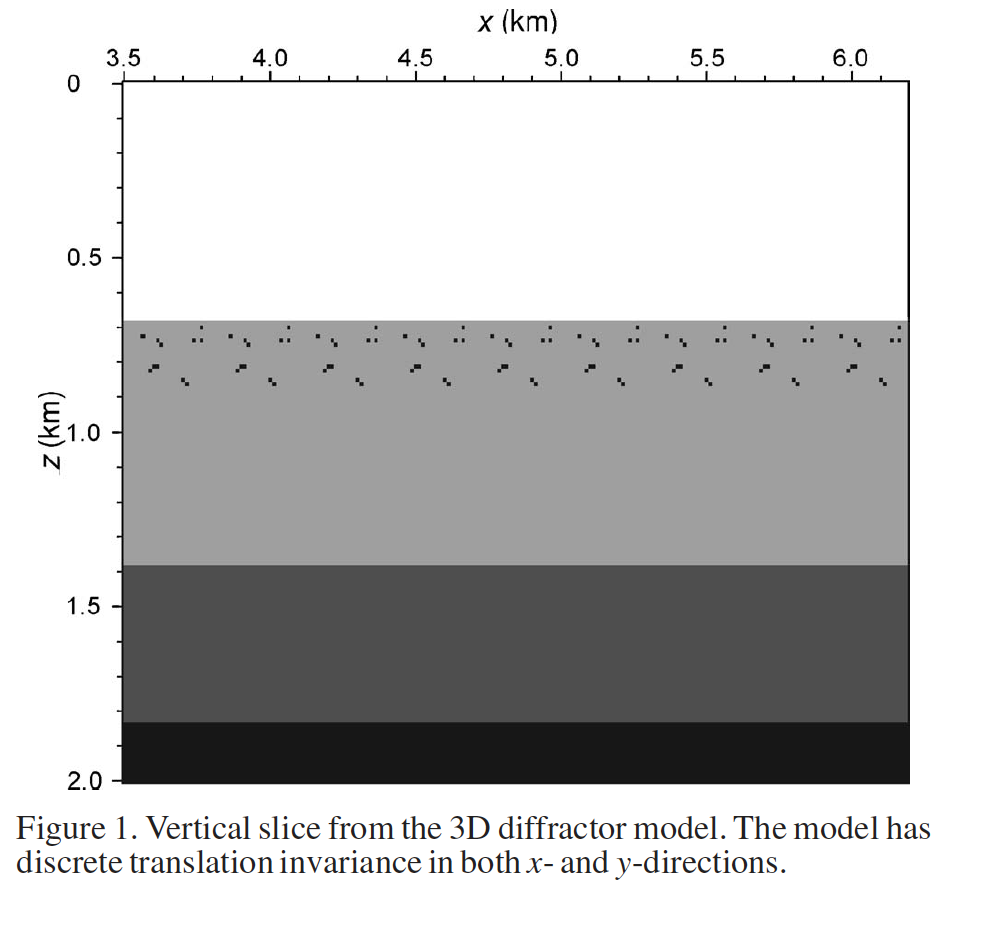
\includegraphics[width=0.8\textwidth]{Fig/fig1.png}
\end{figure}
\end{frame}
%===========================================
\begin{frame}{3D SRME Example}
%===========================================
\begin{figure}
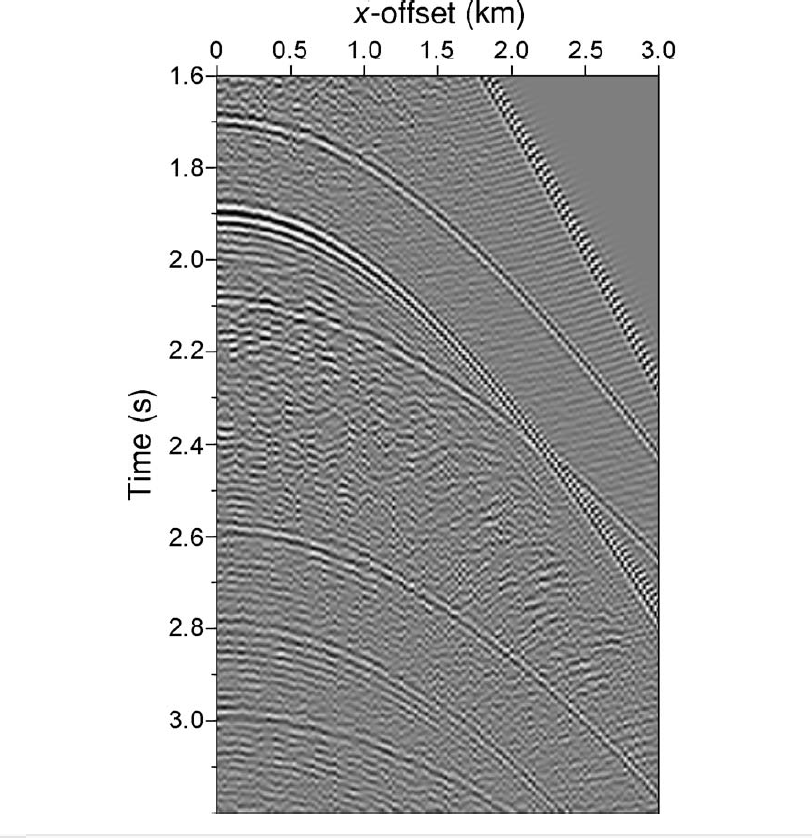
\includegraphics[width=0.7\textwidth]{Fig/fig4.png}
\end{figure}
\end{frame}
%===========================================
\begin{frame}{3D SRME Example}
%===========================================
\begin{figure}
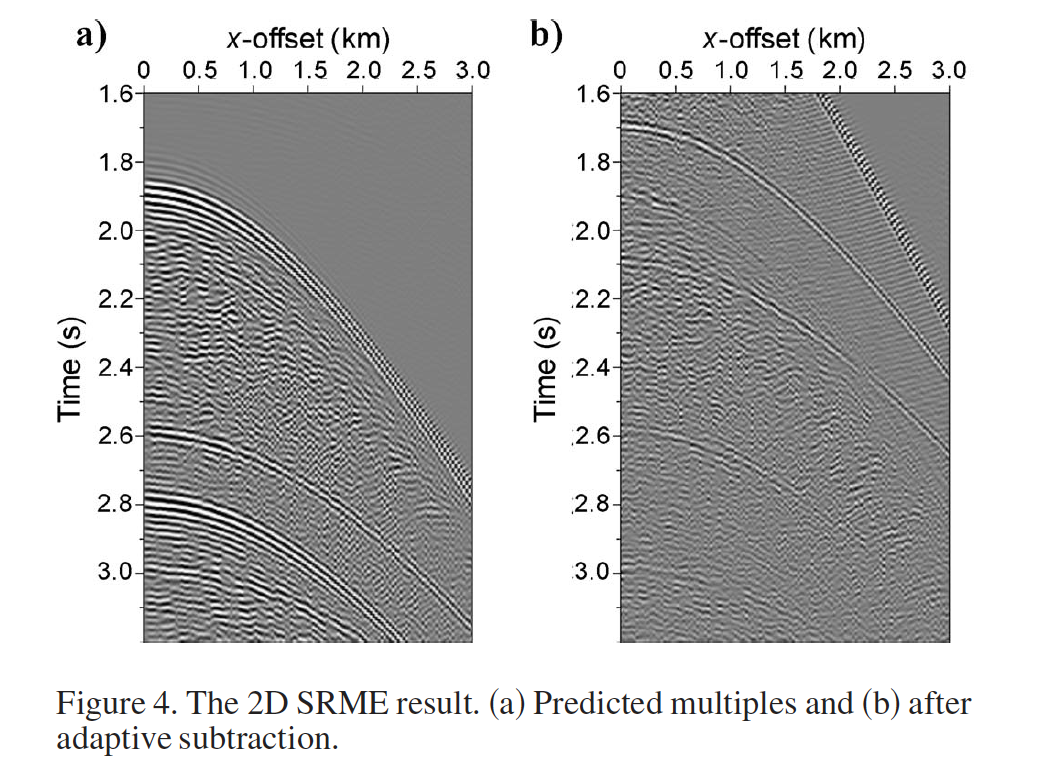
\includegraphics[width=0.8\textwidth]{Fig/fig2.png}
\end{figure}
\end{frame}
%===========================================
\begin{frame}{3D SRME Example}
%===========================================
\begin{figure}
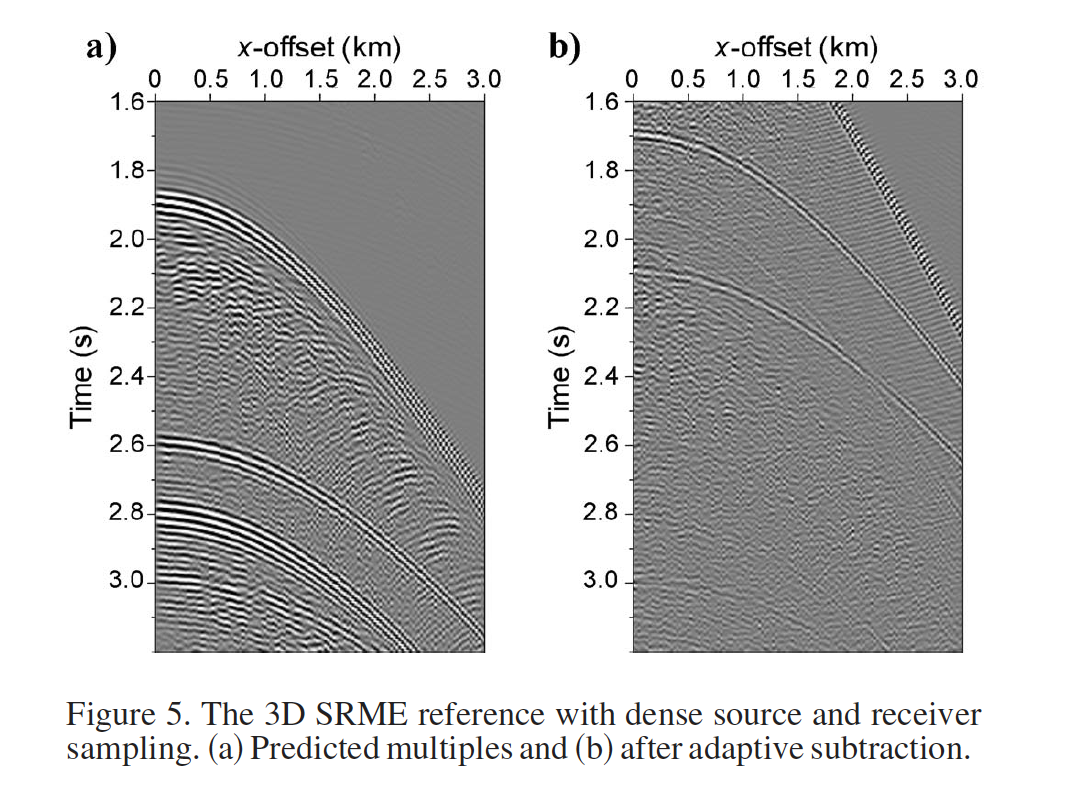
\includegraphics[width=0.8\textwidth]{Fig/fig3.png}
\end{figure}
\end{frame}
%===========================================
\begin{frame}{3D SRME Example}
%===========================================
\begin{figure}
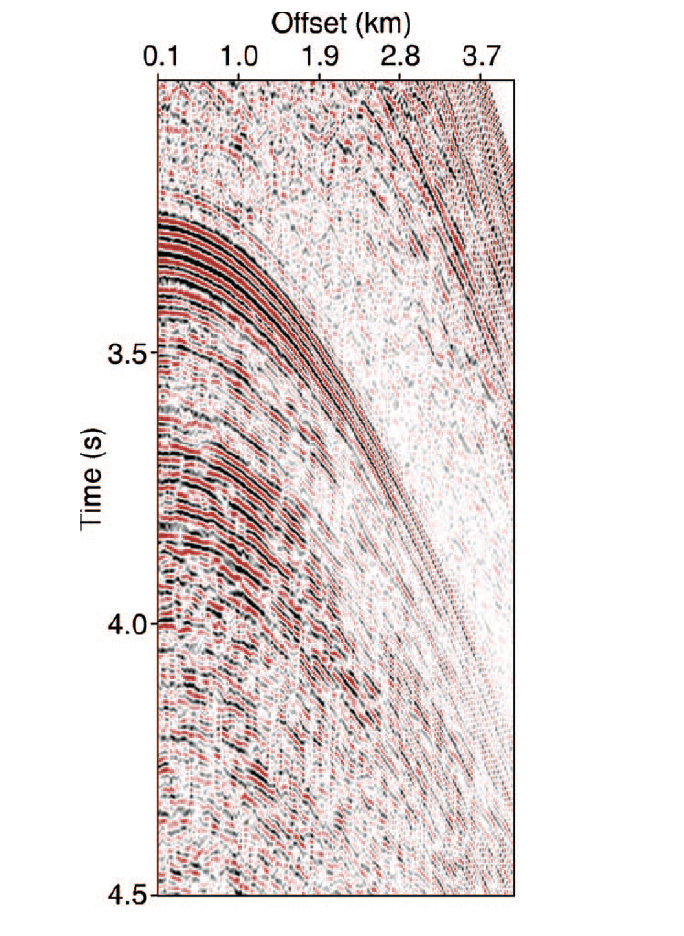
\includegraphics[width=0.5\textwidth]{Fig/fig5.png}
\end{figure}
\end{frame}
%===========================================
\begin{frame}{3D SRME Example}
%===========================================
\begin{figure}
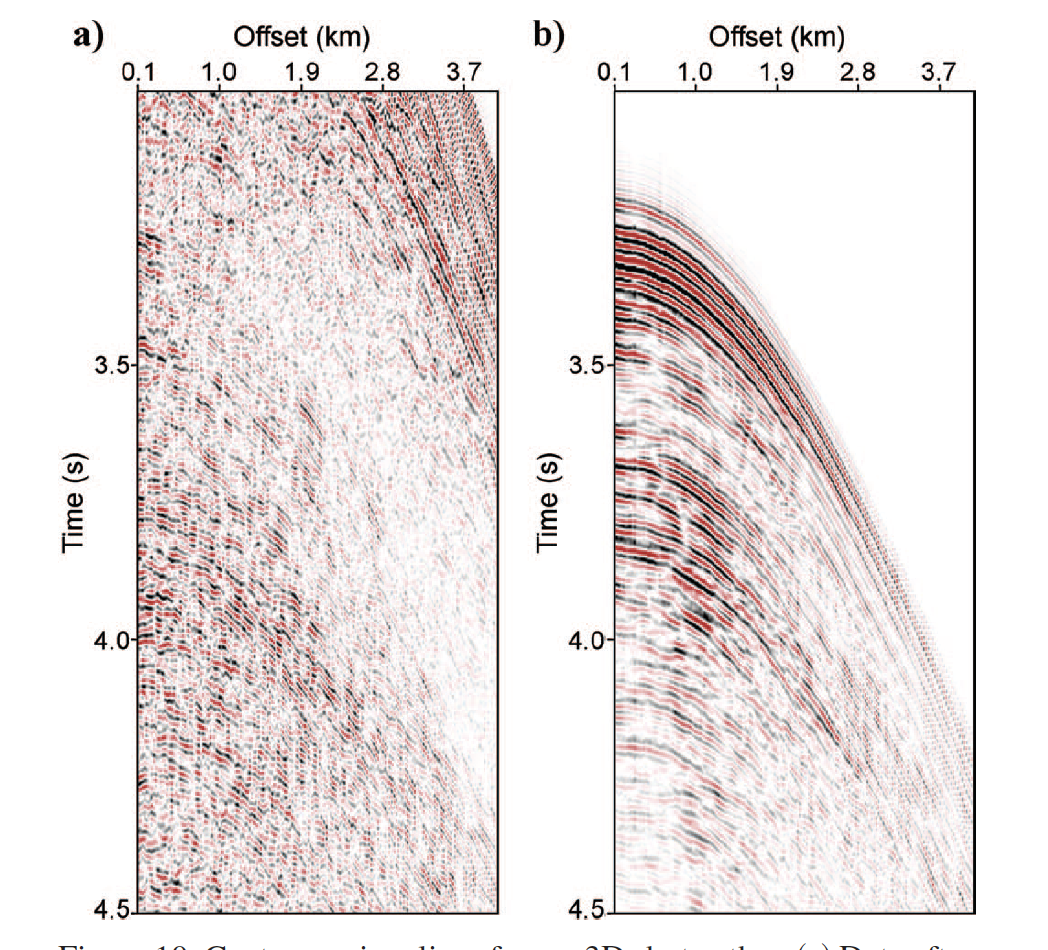
\includegraphics[width=0.7\textwidth]{Fig/fig6.png}
\end{figure}
\end{frame}
%===========================================
\begin{frame}{3D SRME Example}
%===========================================
\begin{figure}
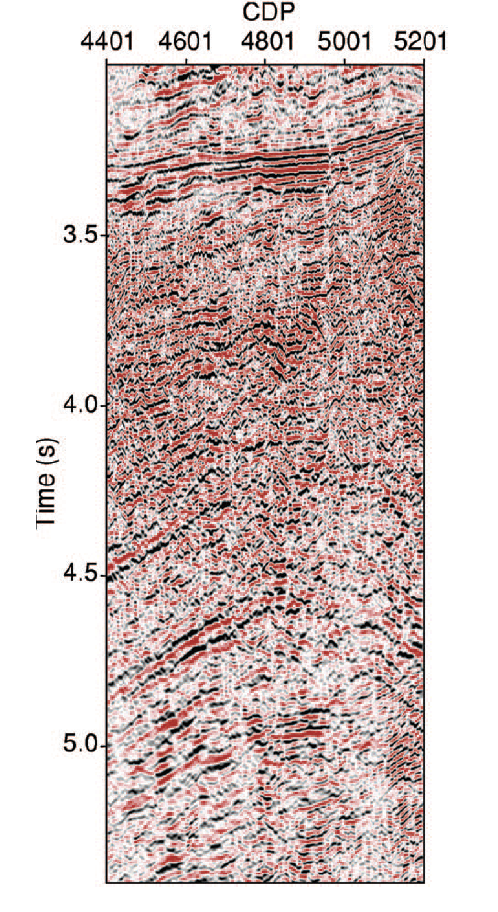
\includegraphics[width=0.4\textwidth]{Fig/fig7.png}
\end{figure}
\end{frame}
%===========================================
\begin{frame}{3D SRME Example}
%===========================================
\begin{figure}
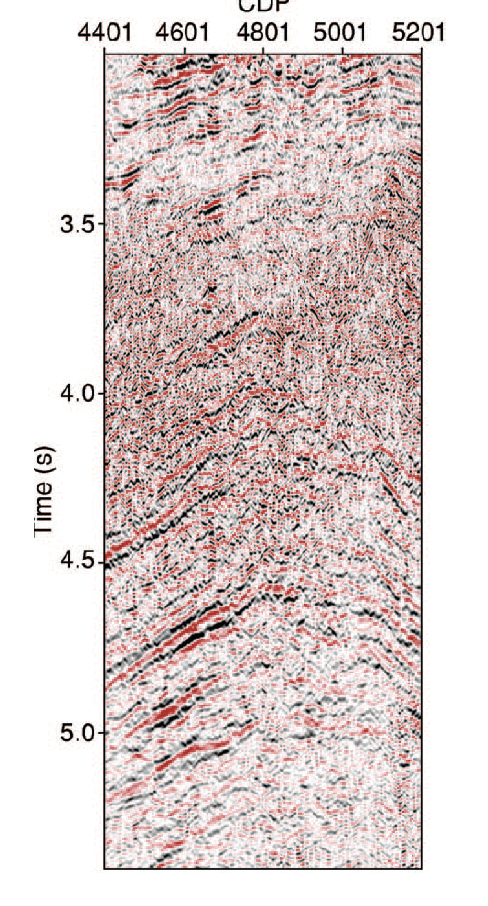
\includegraphics[width=0.4\textwidth]{Fig/fig8.png}
\end{figure}
\end{frame}
%===========================================
\begin{frame}{SRME}
%===========================================
\begin{figure}
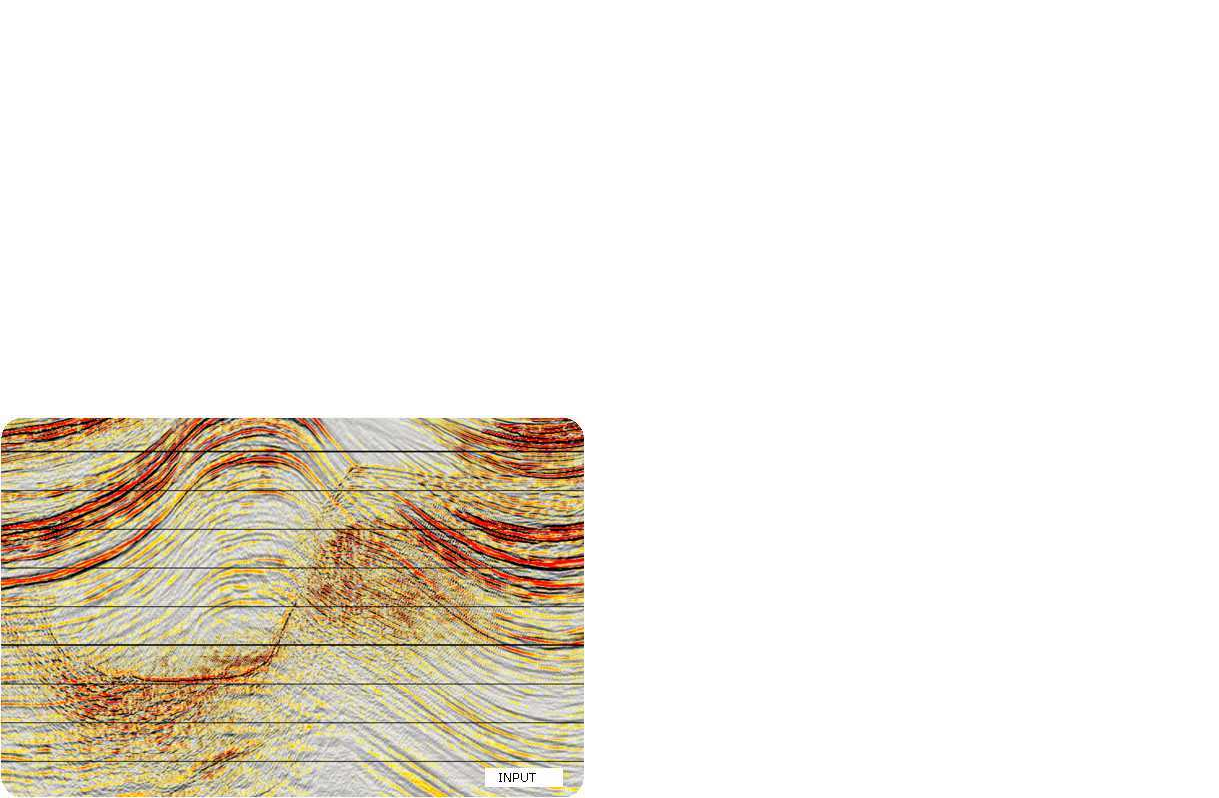
\includegraphics[width=1.0\textwidth]{Fig/ch6-srme1.pdf}
\caption{Data with multiples (Courtesy of CGG)}
\end{figure}
\end{frame}
%===========================================
\begin{frame}
%===========================================
\begin{figure}
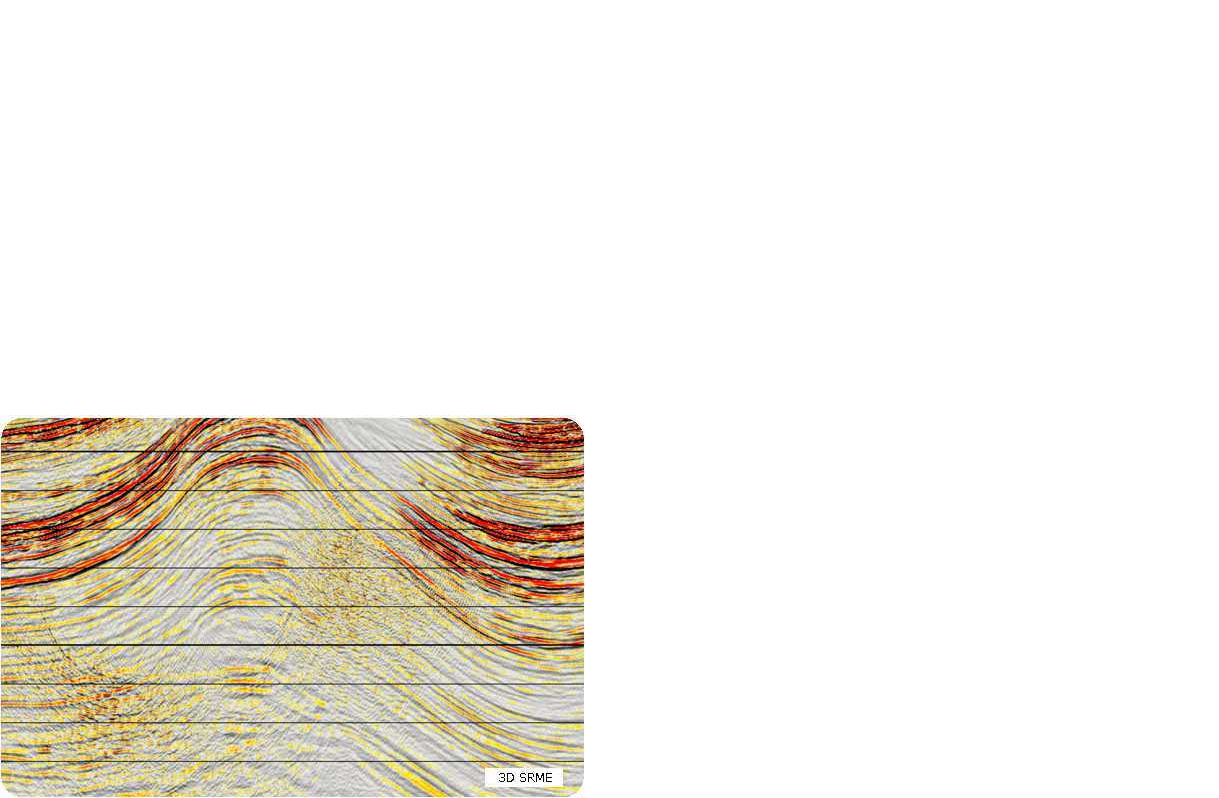
\includegraphics[width=1.0\textwidth]{Fig/ch6-srme2.pdf}
\caption{Multiples removed using SRME (Courtesy of CGG)}
\end{figure}
\end{frame}
%
\end{document}
%
